We now return to the case study outlined in section \ref{sec:casestudy}. We have implemented the simulation in \texttt{Python}, using the \texttt{slugs} reactive synthesis tool~\cite{EhlersR16}. The experiments were performed on an Intel i5-5300U 2.30 GHz CPU with 8 GB of RAM.

 We analyze two scenarios. In Figure \ref{fig:experiment}, we have six available mobile sensors. We compare the surveillance strategy with the situation in Figure \ref{fig:3experiment} where we have three. Our global surveillance task is $\LTLsquare \LTLdiamond p_5$, i.e, we need to infinitely often bring the belief of the target location to 5 cells or lower. 

\begin{figure}
	\centering
\subfloat[The gridworld in \ref{fig:SGR-grid} partitioned into 6 subgames. \label{fig:experiment}]{
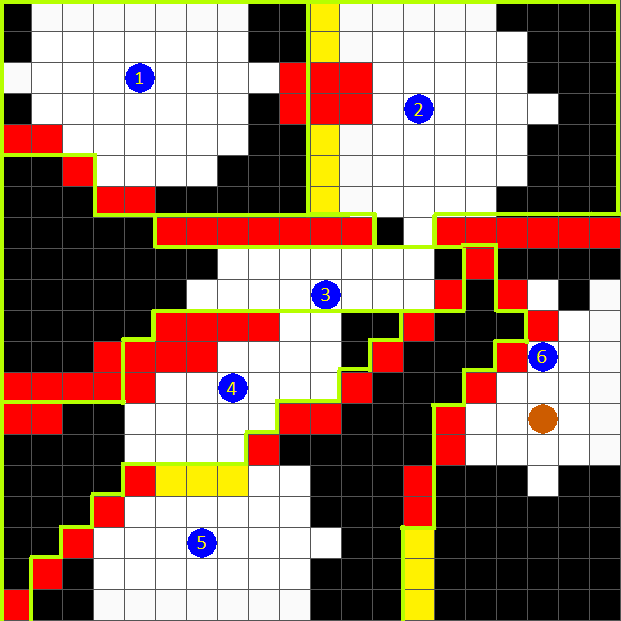
\includegraphics[scale=0.18]{figs/SGR-grid-vis-part.png}
\hspace{1.5cm}}
%\hfill
\subfloat[The gridworld in \ref{fig:SGR-grid} partitioned into 3 subgames. \label{fig:3experiment}]{
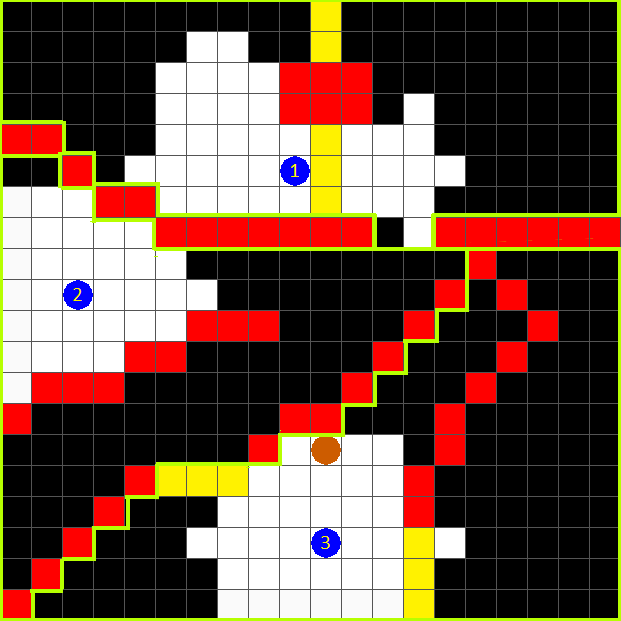
\includegraphics[scale=0.18]{figs/SGR-grid-vis-part_3.png}
\hspace{.3cm}}

\caption{Cases with 6 mobile sensors in Fig \ref{fig:experiment} and 3 mobile sensors in Fig \ref{fig:3experiment}. The mobile sensors are blue circles and the target is represented in orange. The red cells represent impassable terrain (such as dense foliage) that cannot be seen through by the sensors. Black cells are locations not visible to any sensor.}\label{fig:bigexp}\vspace{-0.5cm}
\end{figure} 

Solving either case centralized is not computationally feasible as the state space grows exponentially with the number of sensors - we will have in the order of $400^6$ and $400^3$ states respectively. Thus, we partition the multi-agent surveillance game into subgames as shown in Figures \ref{fig:experiment} and \ref{fig:3experiment}. We then solve each game individually with local specifications $\locspec_i(\square \lozenge p_5)$. We solve these \emph{single-agent} surveillance game using an abstraction-based method detailed in a companion submission to CDC 2018. We refer the reader to \cite{arxiv} for more details on this method. We report the synthesis times in Table \ref{tab:synthtime}.

\begin{table}[h!]
\vspace{-0.2cm}
	\centering
	\caption{Synthesis times for each surveillance subgame}
	\label{tab:synthtime}
	\begin{tabular}{c|l|l|l}
		\multicolumn{1}{l|}{}                                    & \textbf{Subgame} & \textbf{Number of states} & \textbf{Synthesis time (s)} \\ \hline \hline
		\multirow{7}{*}{\textbf{6 sensors}}
		& Subgame 1   & 69     & 101                          \\
	    & Subgame 2   & 74     & 206                          \\
		& Subgame 3   & 62     & 111                          \\
		& Subgame 4   & 52     & 88                          \\
		& Subgame 5   & 77     & 285                          \\
		& Subgame 6   & 66     & 64                          \\ \hline
		& \textbf{Total}   & \textbf{400}         & \textbf{855}                         \\ \hline
		\multicolumn{1}{l|}{\multirow{4}{*}{\textbf{3 sensors}}} & Subgame 1        & 142 & 473                         \\
		\multicolumn{1}{l|}{}                                    & Subgame 2        & 113 & 306                         \\
		\multicolumn{1}{l|}{}                                    & Subgame 3        & 145 & 372                         \\ \hline
		\multicolumn{1}{l|}{}                                    &  \textbf{Total} & \textbf{400}            & \textbf{1151}                        
	\end{tabular}
\end{table}
\vspace{-0.2cm}
The multi-agent surveillance game in Figure \ref{fig:experiment} results in more subgames compared to the game in \ref{fig:experiment}. However, each game is much smaller and strategies can be synthesized faster in each subgame. Figure \ref{fig:case1exp} shows snapshots in time of the simulation of the 3 sensor surveillance game in Figure \ref{fig:3experiment}. The target is being controlled by a human and the sensors are following their synthesized local surveillance strategies. The global belief is depicted in Figure \ref{fig:case1exp} as grey cells, meaning that the combined knowledge of all the sensors has restricted the location of the target into one of the grey cells.
\begin{figure}
	
	\begin{minipage}{5.0cm}
		\centering
		\subfloat[$t_8$ \label{fig:case1t2}]{
			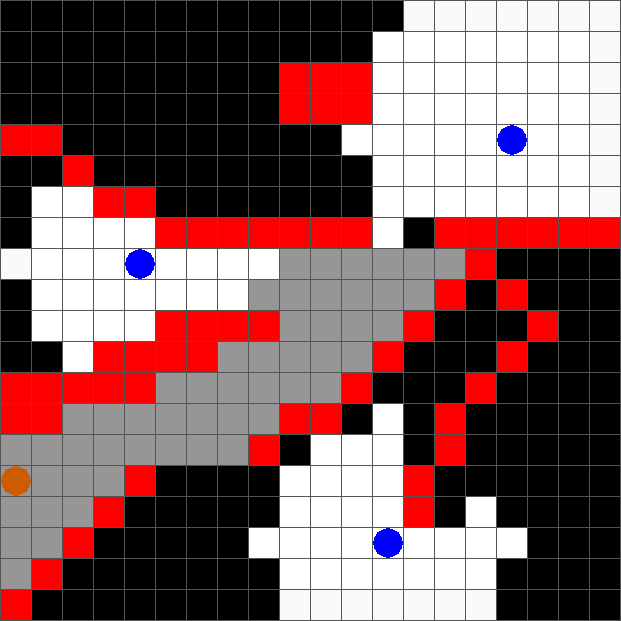
\includegraphics[scale=0.12]{figs/results_t2.png}\hspace{.7cm}
		}
		\subfloat[$t_{12}$ \label{fig:case1t3}]{
			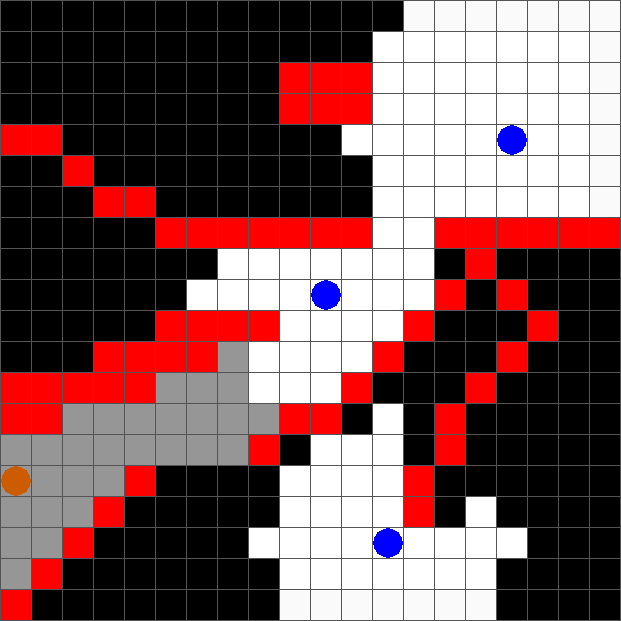
\includegraphics[scale=0.12]{figs/results_t3.png}\hspace{.7cm}
		}
		\subfloat[$t_{16}$ \label{fig:case1t4}]{
			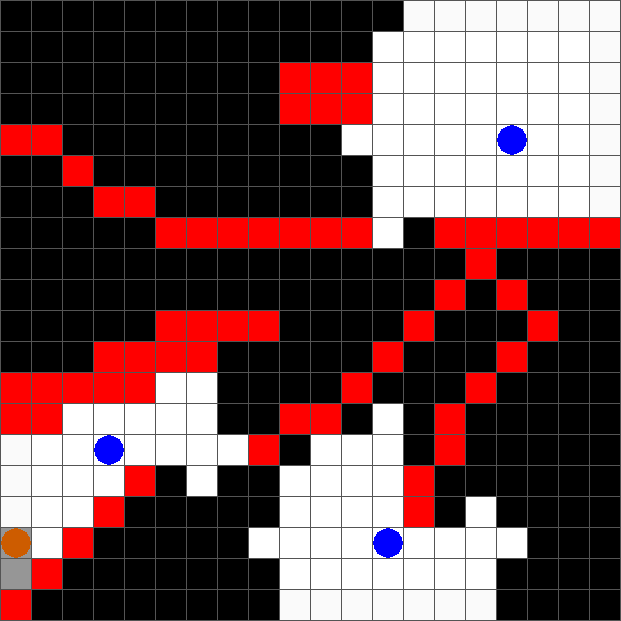
\includegraphics[scale=0.12]{figs/results_t4.png}\hspace{.7cm}
		}
	\end{minipage}
	\begin{minipage}{5.0cm}
		\centering
		\subfloat[$t_{18}$  \label{fig:case1t5}]{
			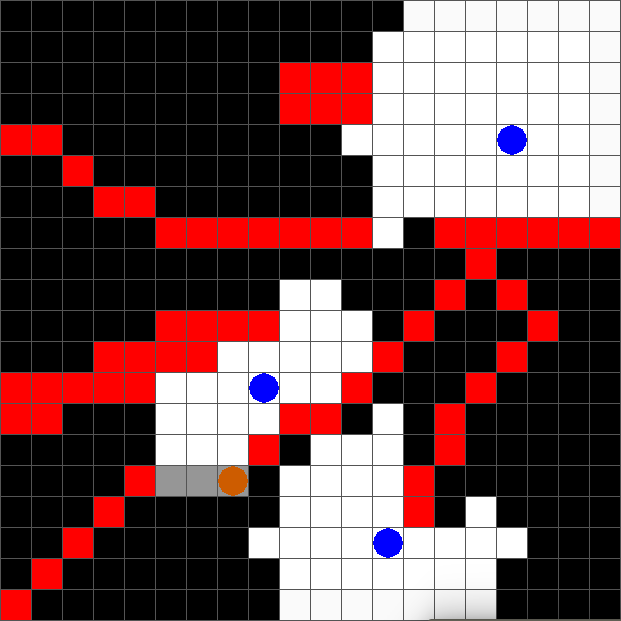
\includegraphics[scale=0.12]{figs/results_t1.png}\hspace{.7cm}
		}
		\subfloat[$t_{20}$ \label{fig:case1t6}]{
			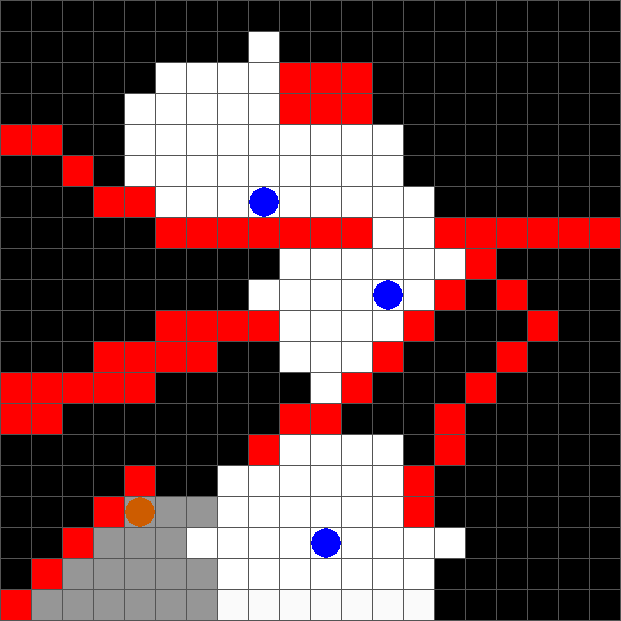
\includegraphics[scale=0.12]{figs/results_t5.png}\hspace{.7cm}
		}
		\subfloat[$t_{22}$ \label{fig:case1t7}]{
			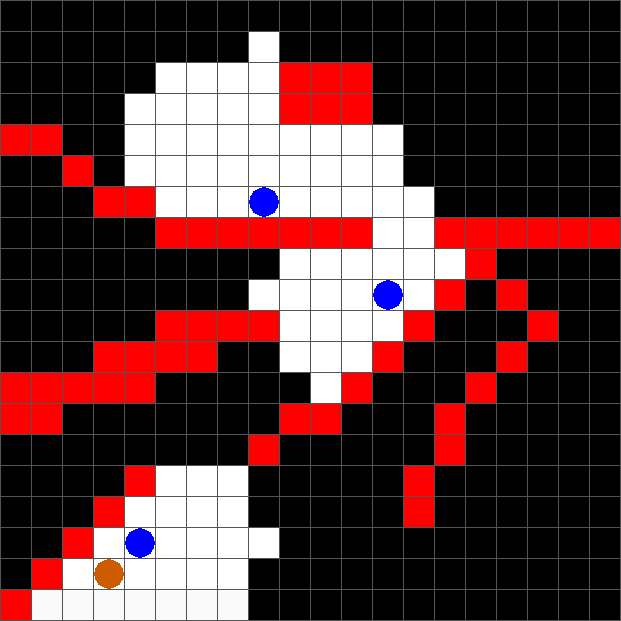
\includegraphics[scale=0.12]{figs/results_t6.png}\hspace{.7cm}
		}
		
	\end{minipage}
	
	
	\caption{Figures \ref{fig:case1t2} - \ref{fig:case1t7} are chronological snapshots at various points in time during the simulation of the surveillance game in Figure \ref{fig:3experiment}. Grey states represent the global belief of the target's location.  
	}\vspace{-0.5cm}
	\label{fig:case1exp}
	
\end{figure}

 We see, in Figures \ref{fig:case1t2} - \ref{fig:case1t4}, that the target is in the subgame corresponding to sensor 2. Hence, only sensor 2 is moving and trying to lower its belief to below 5 cells (which it does in Figure \ref{fig:case1t5}). In Figures \ref{fig:case1t3} - \ref{fig:case1t5}, the target starts moving towards subgame 3 at which point sensor 3 takes over in figures \ref{fig:case1t6} - \ref{fig:case1t7}. There is no communication between any of the agents, and each satisfy only their local surveillance specification. However, our construction guarantees that the global specification of $\square \lozenge p_5$ will be satisfied. %We include a link to a video of the simulation at \url{google.com}
 
 %In figure \ref{fig:case1t2}, the target is in the region of a static sensor. Hence, the global belief is restricted to the region that sensor operates. 